%%%%%%%%%%%%%%%%%%%%%%%%%%%%%%%%%%%%%%%%%%%%%%%%%%%%%%%%%%%%%%%%%%%%%%%%%%%%%%%%
% Modelo para apresentações do Magister
%
% Por: Abrantes Araújo Silva Filho
%      abrantesasf@gmail.com


%%%%%%%%%%%%%%%%%%%%%%%%%%%%%%%%%%%%%%%%%%%%%%%%%%%%%%%%%%%%%%%%%%%%%%%%%%%%%%%%
%%% Classe do documento
\RequirePackage{ifpdf}
\ifpdf
  \pdfminorversion=7
  \documentclass[pdftex, brazil, aspectratio=169]{beamer}
\else
  \documentclass[brazil, aspectratio=169]{beamer}
\fi
\setbeamertemplate{navigation symbols}{}
\usetheme{Magister}
\usefonttheme[onlymath]{serif}


%%%%%%%%%%%%%%%%%%%%%%%%%%%%%%%%%%%%%%%%%%%%%%%%%%%%%%%%%%%%%%%%%%%%%%%%%%%%%%%%
%%% Preâmbulo com todas as outras outras chamadas para todos os outros packages
%%% e o que mais for necessário
%%%%%%%%%%%%%%%%%%%%%%%%%%%%%%%%%%%%%%%%%%%%%%%%%%%%%%%%%%%%%%%%%%%%%%%%%%%%%%%%
% Por: Abrantes Araújo Silva Filho
%      abrantesasf@gmail.com
% URL: https://github.com/abrantesasf/latex


%%%%%%%%%%%%%%%%%%%%%%%%%%%%%%%%%%%%%%%%%%%%%%%%%%%%%%%%%%%%%%%%%%%%%%%%%%%%%%%%
%%% Compilação condicional em PDF
%%%%%%%%%%%%%%%%%%%%%%%%%%%%%%%%%%%%%%%%%%%%%%%%%%%%%%%%%%%%%%%%%%%%%%%%%%%%%%%%
% Por: Abrantes Araújo Silva Filho
%      abrantesasf@gmail.com
% URL: https://github.com/abrantesasf/latex


%%%%%%%%%%%%%%%%%%%%%%%%%%%%%%%%%%%%%%%%%%%%%%%%%%%%%%%%%%%%%%%%%%%%%%%%%%%%%%%%
%%% Pacote para compilaçãocondicional em PDF
\usepackage{ifpdf}


%%%%%%%%%%%%%%%%%%%%%%%%%%%%%%%%%%%%%%%%%%%%%%%%%%%%%%%%%%%%%%%%%%%%%%%%%%%%%%%%
%%% Estruturas de controle
%%%%%%%%%%%%%%%%%%%%%%%%%%%%%%%%%%%%%%%%%%%%%%%%%%%%%%%%%%%%%%%%%%%%%%%%%%%%%%%%
% Por: Abrantes Araújo Silva Filho
%      abrantesasf@gmail.com
% URL: https://github.com/abrantesasf/latex


%%%%%%%%%%%%%%%%%%%%%%%%%%%%%%%%%%%%%%%%%%%%%%%%%%%%%%%%%%%%%%%%%%%%%%%%%%%%%%%%
%%% Carrega pacotes iniciais necessários para estrutura de controle e para a
%%% criação e o parse de novos comandos
\usepackage{ifthen}
\usepackage{xparse}



%%%%%%%%%%%%%%%%%%%%%%%%%%%%%%%%%%%%%%%%%%%%%%%%%%%%%%%%%%%%%%%%%%%%%%%%%%%%%%%%
%%% Configurações de layout da página
%%%%%%%%%%%%%%%%%%%%%%%%%%%%%%%%%%%%%%%%%%%%%%%%%%%%%%%%%%%%%%%%%%%%%%%%%%%%%%%%
% Por: Abrantes Araújo Silva Filho
%      abrantesasf@gmail.com
% URL: https://github.com/abrantesasf/latex


%%%%%%%%%%%%%%%%%%%%%%%%%%%%%%%%%%%%%%%%%%%%%%%%%%%%%%%%%%%%%%%%%%%%%%%%%%%%%%%%
%%% Configuração do tamanho da página, margens, espaçamento entrelinhas e, se
%%% necessário, ativa a indentação dos primeiros parágrafos.
\makeatletter
\@ifclassloaded{beamer}{}{
\ifpdf
  \usepackage[pdftex]{geometry}
\else
  \usepackage[dvips]{geometry}
\fi
}
\makeatother

\usepackage{setspace}


%%%%%%%%%%%%%%%%%%%%%%%%%%%%%%%%%%%%%%%%%%%%%%%%%%%%%%%%%%%%%%%%%%%%%%%%%%%%%%%%
%%% Cabeçalho e rodapé
%%%%%%%%%%%%%%%%%%%%%%%%%%%%%%%%%%%%%%%%%%%%%%%%%%%%%%%%%%%%%%%%%%%%%%%%%%%%%%%%%
% Por: Abrantes Araújo Silva Filho
%      abrantesasf@gmail.com
% URL: https://github.com/abrantesasf/latex


%%%%%%%%%%%%%%%%%%%%%%%%%%%%%%%%%%%%%%%%%%%%%%%%%%%%%%%%%%%%%%%%%%%%%%%%%%%%%%%%
%%% Configurações de cabeçalho e rodapé:
%%% Atenção: é MUITO DIFÍCIL ajustar apropriadamente os running header
%%% e footer da primeira vez. Você pode confiar no LaTeX e deixar que
%%% ele faça o ajuste automaticamente ou pode quebrar a cabeça e
%%% tentar melhorar algo que o LaTeX já faz muito bem. O que você
%%% perfere?
\usepackage{fancyhdr}
\setlength{\headheight}{1cm}
\setlength{\footskip}{1.5cm}
\renewcommand{\headrulewidth}{0.3pt}
\renewcommand{\footrulewidth}{0.0pt}
\pagestyle{fancy}
\renewcommand{\sectionmark}[1]{%
  \markboth{\uppercase{#1}}{}}
\renewcommand{\subsectionmark}[1]{%
  \markright{\uppercase{\thesubsection \hspace{0.1cm} #1}}{}}
\fancyhead{}
\fancyfoot{}
\newcommand{\diminuifonte}{%
    \fontsize{9pt}{9}\selectfont
}
\newcommand{\aumentafonte}{%
    \fontsize{12}{12}\selectfont
}
% Configura cabeçalho e rodapé para documentos TWOSIDE
\fancyhead[EL]{\textbf{\thepage}}
\fancyhead[EC]{}
\fancyhead[ER]{\diminuifonte \textbf{\leftmark}}
\fancyhead[OR]{\textbf{\thepage}}
\fancyhead[OC]{}
\fancyhead[OL]{\diminuifonte \textbf{\rightmark}}
\fancyfoot[EL,EC,ER,OR,OC,OL]{}
% Configura cabeçalho e rodapé para documentos ONESIDE
%%\lhead{ \fancyplain{}{sup esquerdo} }
%%\chead{ \fancyplain{}{sup centro} }
%%\rhead{ \fancyplain{}{\thesection} }
%%\lfoot{ \fancyplain{}{inf esquerdo} }
%%\cfoot{ \fancyplain{}{inf centro} }
%%\rfoot{ \fancyplain{}{\thepage} }


%%%%%%%%%%%%%%%%%%%%%%%%%%%%%%%%%%%%%%%%%%%%%%%%%%%%%%%%%%%%%%%%%%%%%%%%%%%%%%%%
%%% Fontes
%%%%%%%%%%%%%%%%%%%%%%%%%%%%%%%%%%%%%%%%%%%%%%%%%%%%%%%%%%%%%%%%%%%%%%%%%%%%%%%%
% Por: Abrantes Araújo Silva Filho
%      abrantesasf@gmail.com
% URL: https://github.com/abrantesasf/latex


%%%%%%%%%%%%%%%%%%%%%%%%%%%%%%%%%%%%%%%%%%%%%%%%%%%%%%%%%%%%%%%%%%%%%%%%%%%%%%%%
%%% Configurações de encoding, lingua e fontes:
\usepackage[T1]{fontenc}
\usepackage[utf8]{inputenc}

% Altera a fonte padrão do documento (nem todas funcionam em modo math):
%   phv = Helvetica
%   ptm = Times
%   ppl = Palatino
%   pbk = bookman
%   pag = AdobeAvantGarde
%   pnc = Adobe NewCenturySchoolBook
\renewcommand{\familydefault}{ppl}


%%%%%%%%%%%%%%%%%%%%%%%%%%%%%%%%%%%%%%%%%%%%%%%%%%%%%%%%%%%%%%%%%%%%%%%%%%%%%%%%
%%% Linguagem e hifenização
%%%%%%%%%%%%%%%%%%%%%%%%%%%%%%%%%%%%%%%%%%%%%%%%%%%%%%%%%%%%%%%%%%%%%%%%%%%%%%%%
% Por: Abrantes Araújo Silva Filho
%      abrantesasf@gmail.com
% URL: https://github.com/abrantesasf/latex


%%%%%%%%%%%%%%%%%%%%%%%%%%%%%%%%%%%%%%%%%%%%%%%%%%%%%%%%%%%%%%%%%%%%%%%%%%%%%%%%
%%% Configurações de linguagem e hifenização
\usepackage[brazil]{babel}

%%%%%%%%%%%%%%%%%%%%%%%%%%%%%%%%%%%%%%%%%%%%%%%%%%%%%%%%%%%%%%%%%%%%%%%%%%%%%%%%
%%% Hifenização específica quando o LaTeX/Babel não conseguirem hifenizar:
\babelhyphenation{Git-Hub}


%%%%%%%%%%%%%%%%%%%%%%%%%%%%%%%%%%%%%%%%%%%%%%%%%%%%%%%%%%%%%%%%%%%%%%%%%%%%%%%%
%%% Matemática
%%%%%%%%%%%%%%%%%%%%%%%%%%%%%%%%%%%%%%%%%%%%%%%%%%%%%%%%%%%%%%%%%%%%%%%%%%%%%%%%
% Por: Abrantes Araújo Silva Filho
%      abrantesasf@gmail.com
% URL: https://github.com/abrantesasf/latex


%%%%%%%%%%%%%%%%%%%%%%%%%%%%%%%%%%%%%%%%%%%%%%%%%%%%%%%%%%%%%%%%%%%%%%%%%%%%%%%%
%%% Carrega bibliotecas e símbolos matemáticos, fontes adicionais e configura
%%% algumas outras opções
\usepackage{amsmath}
\usepackage{amssymb}
\usepackage{amsthm}
\usepackage{amsfonts}
\usepackage{siunitx}
  \sisetup{group-separator = {.}}
  \sisetup{group-digits = {true}}
  \sisetup{output-decimal-marker = {,}}
\usepackage{bm}
\usepackage{cancel}

% Altera separador decimal via comando, se necessário (prefira o siunitx):
%\mathchardef\period=\mathcode`.
%\DeclareMathSymbol{.}{\mathord}{letters}{"3B}

\usepackage{esvect}
\usepackage{mathtools}

%%%%%%%%%%%%%%%%%%%%%%%%%%%%%%%%%%%%%%%%%%%%%%%%%%%%%%%%%%%%%%%%%%%%%%%%%%%%%%%%
%%% Definições para teoremas, etc.
\makeatletter
\@ifclassloaded{article}{
\theoremstyle{definition}
\newtheorem{definicao}{Definição}[section]
\newtheorem{conjecture}{Conjectura}[section]
\newtheorem{teorema}{Teorema}[section]
\newtheorem{lemma}{Lema}[section]
\newtheorem{corolario}{Corolario}[section]
\theoremstyle{remark}
\newtheorem*{nota}{Nota}
\newtheorem*{observacao}{Observação:}
}{}
\@ifclassloaded{book}{
\theoremstyle{definition}
\newtheorem{definicao}{Definição}[chapter]
\newtheorem{conjecture}{Conjectura}[chapter]
\newtheorem{teorema}{Teorema}[chapter]
\newtheorem{lemma}{Lema}[chapter]
\newtheorem{corolario}{Corolario}[chapter]
\theoremstyle{remark}
\newtheorem*{nota}{Nota}
\newtheorem*{observacao}{Observação:}
}{}
\makeatother


%%%%%%%%%%%%%%%%%%%%%%%%%%%%%%%%%%%%%%%%%%%%%%%%%%%%%%%%%%%%%%%%%%%%%%%%%%%%%%%%
%%% Sumário
%%%%%%%%%%%%%%%%%%%%%%%%%%%%%%%%%%%%%%%%%%%%%%%%%%%%%%%%%%%%%%%%%%%%%%%%%%%%%%%%
% Por: Abrantes Araújo Silva Filho
%      abrantesasf@gmail.com
% URL: https://github.com/abrantesasf/latex


%%%%%%%%%%%%%%%%%%%%%%%%%%%%%%%%%%%%%%%%%%%%%%%%%%%%%%%%%%%%%%%%%%%%%%%%%%%%%%%%
%%% Ajustes de sumário
\makeatletter
\@ifclassloaded{article}{
\usepackage[nottoc]{tocbibind}
}{}
\@ifclassloaded{book}{
\usepackage{tocbibind}
}{}
\makeatother


%%%%%%%%%%%%%%%%%%%%%%%%%%%%%%%%%%%%%%%%%%%%%%%%%%%%%%%%%%%%%%%%%%%%%%%%%%%%%%%%
%%% Referências cruzadas, links, citações
%%%%%%%%%%%%%%%%%%%%%%%%%%%%%%%%%%%%%%%%%%%%%%%%%%%%%%%%%%%%%%%%%%%%%%%%%%%%%%%%
% Por: Abrantes Araújo Silva Filho
%      abrantesasf@gmail.com
% URL: https://github.com/abrantesasf/latex


%%%%%%%%%%%%%%%%%%%%%%%%%%%%%%%%%%%%%%%%%%%%%%%%%%%%%%%%%%%%%%%%%%%%%%%%%%%%%%%%%
%%% Carrega pacotes para referências cruzadas, citações dentro do documento,
%%% links para internet e outros.Configura algumas opções.
%%% Não altere a ordem de carregamento dos packages.
\usepackage{varioref}
\ifpdf
  \usepackage[pdftex]{hyperref}
    \hypersetup{
      % Configurações padrão que eu gosto
      unicode=true,
      pdflang={pt-BR},
      bookmarksopen=true,
      bookmarksnumbered=true,
      bookmarksopenlevel=5,
      pdfdisplaydoctitle=true,
      pdfpagemode=UseOutlines,
      pdfstartview=FitH,
      pdfcreator={LaTeX with hyperref package},
      pdfproducer={pdfTeX},
      pdfnewwindow=true,
      colorlinks=true,
      citecolor=red,
      linkcolor=red,
      filecolor=cyan,
      urlcolor=blue
    }
\else
  \usepackage{hyperref}
\fi
\usepackage{cleveref}
\usepackage{url}


%%%%%%%%%%%%%%%%%%%%%%%%%%%%%%%%%%%%%%%%%%%%%%%%%%%%%%%%%%%%%%%%%%%%%%%%%%%%%%%%
%%% Referências bibliográficas
%%%%%%%%%%%%%%%%%%%%%%%%%%%%%%%%%%%%%%%%%%%%%%%%%%%%%%%%%%%%%%%%%%%%%%%%%%%%%%%%
%%% Referências bibliográficas
\usepackage[round, semicolon, authoryear]{natbib}
%\bibliographystyle{natdin}
\bibliographystyle{abrantesasf}


%%%%%%%%%%%%%%%%%%%%%%%%%%%%%%%%%%%%%%%%%%%%%%%%%%%%%%%%%%%%%%%%%%%%%%%%%%%%%%%%
%%% Glossário e índice remissivo
%%%%%%%%%%%%%%%%%%%%%%%%%%%%%%%%%%%%%%%%%%%%%%%%%%%%%%%%%%%%%%%%%%%%%%%%%%%%%%%%
%%% Pacotes para glossário e índice remissivo
\usepackage{makeidx}
\makeindex

\usepackage[toc]{glossaries}
\newglossary[nlg]{notation}{not}{ntn}{Notação}

\newglossaryentry{not:set}{
type = notation,
name = {$\mathbb{N}$},
description = conjunto dos números naturais,
sort = {N}}

\makeglossaries


%%%%%%%%%%%%%%%%%%%%%%%%%%%%%%%%%%%%%%%%%%%%%%%%%%%%%%%%%%%%%%%%%%%%%%%%%%%%%%%%
%%% Computação
%%%%%%%%%%%%%%%%%%%%%%%%%%%%%%%%%%%%%%%%%%%%%%%%%%%%%%%%%%%%%%%%%%%%%%%%%%%%%%%%
% Por: Abrantes Araújo Silva Filho
%      abrantesasf@gmail.com
% URL: https://github.com/abrantesasf/latex


%%%%%%%%%%%%%%%%%%%%%%%%%%%%%%%%%%%%%%%%%%%%%%%%%%%%%%%%%%%%%%%%%%%%%%%%%%%%%%%%
%%% Carrega packages relacionados à computação
\usepackage{algorithm2e}
\usepackage{algorithmicx}
\usepackage{algpseudocode}
\usepackage{listings}
  \lstset{literate=
    {á}{{\'a}}1 {é}{{\'e}}1 {í}{{\'i}}1 {ó}{{\'o}}1 {ú}{{\'u}}1
    {Á}{{\'A}}1 {É}{{\'E}}1 {Í}{{\'I}}1 {Ó}{{\'O}}1 {Ú}{{\'U}}1
    {à}{{\`a}}1 {è}{{\`e}}1 {ì}{{\`i}}1 {ò}{{\`o}}1 {ù}{{\`u}}1
    {À}{{\`A}}1 {È}{{\'E}}1 {Ì}{{\`I}}1 {Ò}{{\`O}}1 {Ù}{{\`U}}1
    {ä}{{\"a}}1 {ë}{{\"e}}1 {ï}{{\"i}}1 {ö}{{\"o}}1 {ü}{{\"u}}1
    {Ä}{{\"A}}1 {Ë}{{\"E}}1 {Ï}{{\"I}}1 {Ö}{{\"O}}1 {Ü}{{\"U}}1
    {â}{{\^a}}1 {ê}{{\^e}}1 {î}{{\^i}}1 {ô}{{\^o}}1 {û}{{\^u}}1
    {Â}{{\^A}}1 {Ê}{{\^E}}1 {Î}{{\^I}}1 {Ô}{{\^O}}1 {Û}{{\^U}}1
    {œ}{{\oe}}1 {Œ}{{\OE}}1 {æ}{{\ae}}1 {Æ}{{\AE}}1 {ß}{{\ss}}1
    {ű}{{\H{u}}}1 {Ű}{{\H{U}}}1 {ő}{{\H{o}}}1 {Ő}{{\H{O}}}1
    {ç}{{\c c}}1 {Ç}{{\c C}}1 {ø}{{\o}}1 {å}{{\r a}}1 {Å}{{\r A}}1
    {€}{{\euro}}1 {£}{{\pounds}}1 {«}{{\guillemotleft}}1
    {»}{{\guillemotright}}1 {ñ}{{\~n}}1 {Ñ}{{\~N}}1 {¿}{{?`}}1
  }


%%%%%%%%%%%%%%%%%%%%%%%%%%%%%%%%%%%%%%%%%%%%%%%%%%%%%%%%%%%%%%%%%%%%%%%%%%%%%%%%
%%% Cores
%%%%%%%%%%%%%%%%%%%%%%%%%%%%%%%%%%%%%%%%%%%%%%%%%%%%%%%%%%%%%%%%%%%%%%%%%%%%%%%%
% Por: Abrantes Araújo Silva Filho
%      abrantesasf@gmail.com
% URL: https://github.com/abrantesasf/latex


%%%%%%%%%%%%%%%%%%%%%%%%%%%%%%%%%%%%%%%%%%%%%%%%%%%%%%%%%%%%%%%%%%%%%%%%%%%%%%%%
%%% Ativa suporte extendido a cores
\makeatletter
\@ifclassloaded{beamer}{
  \usepackage{xcolor} % Opções de cores: usenames (16), dvipsnames (64),
                      % svgnames (150) e x11names (300).
}{
  \usepackage[svgnames]{xcolor} % Opções de cores: usenames (16), dvipsnames (64),
                                % svgnames (150) e x11names (300).
}
\makeatother


%%%%%%%%%%%%%%%%%%%%%%%%%%%%%%%%%%%%%%%%%%%%%%%%%%%%%%%%%%%%%%%%%%%%%%%%%%%%%%%%
%%% Gráficos
%%%%%%%%%%%%%%%%%%%%%%%%%%%%%%%%%%%%%%%%%%%%%%%%%%%%%%%%%%%%%%%%%%%%%%%%%%%%%%%%
% Por: Abrantes Araújo Silva Filho
%      abrantesasf@gmail.com
% URL: https://github.com/abrantesasf/latex


%%%%%%%%%%%%%%%%%%%%%%%%%%%%%%%%%%%%%%%%%%%%%%%%%%%%%%%%%%%%%%%%%%%%%%%%%%%%%%%%
%%% Suporte à importação de gráficos externos
%\usepackage{tcolorbox}
\ifpdf
  \usepackage[pdftex]{graphicx}
\else
  \usepackage[dvips]{graphicx}
\fi

%%%%%%%%%%%%%%%%%%%%%%%%%%%%%%%%%%%%%%%%%%%%%%%%%%%%%%%%%%%%%%%%%%%%%%%%%%%%%%%%
%%% Suporte à criação de gráficos proceduralmente no LaTeX:
\usepackage{tikz}
\usetikzlibrary{arrows,automata,backgrounds,matrix,patterns,positioning,shapes,shadows}



%%%%%%%%%%%%%%%%%%%%%%%%%%%%%%%%%%%%%%%%%%%%%%%%%%%%%%%%%%%%%%%%%%%%%%%%%%%%%%%%
%%% Ícones
%%%%%%%%%%%%%%%%%%%%%%%%%%%%%%%%%%%%%%%%%%%%%%%%%%%%%%%%%%%%%%%%%%%%%%%%%%%%%%%%
% Por: Abrantes Araújo Silva Filho
%      abrantesasf@gmail.com
% URL: https://github.com/abrantesasf/latex


%%%%%%%%%%%%%%%%%%%%%%%%%%%%%%%%%%%%%%%%%%%%%%%%%%%%%%%%%%%%%%%%%%%%%%%%%%%%%%%%
%%% Pacotes com ícones, figuras e gráficos extras

% Ícones da Creative Commons:
\usepackage{ccicons}


%%%%%%%%%%%%%%%%%%%%%%%%%%%%%%%%%%%%%%%%%%%%%%%%%%%%%%%%%%%%%%%%%%%%%%%%%%%%%%%%
%%% Blocos
%%%%%%%%%%%%%%%%%%%%%%%%%%%%%%%%%%%%%%%%%%%%%%%%%%%%%%%%%%%%%%%%%%%%%%%%%%%%%%%%
% Por: Abrantes Araújo Silva Filho
%      abrantesasf@gmail.com
% URL: https://github.com/abrantesasf/latex


%%%%%%%%%%%%%%%%%%%%%%%%%%%%%%%%%%%%%%%%%%%%%%%%%%%%%%%%%%%%%%%%%%%%%%%%%%%%%%%%
%%% Ambiente para boxes em posições arbitrárias

\makeatletter
\@ifclassloaded{beamer}{
  \usepackage{textpos}
}{}
\makeatother


%%%%%%%%%%%%%%%%%%%%%%%%%%%%%%%%%%%%%%%%%%%%%%%%%%%%%%%%%%%%%%%%%%%%%%%%%%%%%%%%
%%% Boxes coloridos
%%%%%%%%%%%%%%%%%%%%%%%%%%%%%%%%%%%%%%%%%%%%%%%%%%%%%%%%%%%%%%%%%%%%%%%%%%%%%%%%
% Por: Abrantes Araújo Silva Filho
%      abrantesasf@gmail.com
% URL: https://github.com/abrantesasf/latex


%%%%%%%%%%%%%%%%%%%%%%%%%%%%%%%%%%%%%%%%%%%%%%%%%%%%%%%%%%%%%%%%%%%%%%%%%%%%%%%%
%%% Ativa suporte para boxes coloridos
\usepackage[most]{tcolorbox}


%%%%%%%%%%%%%%%%%%%%%%%%%%%%%%%%%%%%%%%%%%%%%%%%%%%%%%%%%%%%%%%%%%%%%%%%%%%%%%%%
%%% Tabelas
%%%%%%%%%%%%%%%%%%%%%%%%%%%%%%%%%%%%%%%%%%%%%%%%%%%%%%%%%%%%%%%%%%%%%%%%%%%%%%%%
% Por: Abrantes Araújo Silva Filho
%      abrantesasf@gmail.com
% URL: https://github.com/abrantesasf/latex


%%%%%%%%%%%%%%%%%%%%%%%%%%%%%%%%%%%%%%%%%%%%%%%%%%%%%%%%%%%%%%%%%%%%%%%%%%%%%%%%
%%% Packages para tabelas
\usepackage{array}
\usepackage{longtable}
\usepackage{tabularx}
\usepackage{tabu}
\usepackage{lscape}
\usepackage{colortbl}  
\usepackage{booktabs}


%%%%%%%%%%%%%%%%%%%%%%%%%%%%%%%%%%%%%%%%%%%%%%%%%%%%%%%%%%%%%%%%%%%%%%%%%%%%%%%%
%%% Ambientes de listas
%%%%%%%%%%%%%%%%%%%%%%%%%%%%%%%%%%%%%%%%%%%%%%%%%%%%%%%%%%%%%%%%%%%%%%%%%%%%%%%%
% Por: Abrantes Araújo Silva Filho
%      abrantesasf@gmail.com
% URL: https://github.com/abrantesasf/latex


%%%%%%%%%%%%%%%%%%%%%%%%%%%%%%%%%%%%%%%%%%%%%%%%%%%%%%%%%%%%%%%%%%%%%%%%%%%%%%%%
%%% Packages para ambientes de listas
\makeatletter
\@ifclassloaded{beamer}{
  \usepackage{listings}
}{
  \usepackage{enumitem}
  \usepackage[ampersand]{easylist}
}
\makeatother



%%%%%%%%%%%%%%%%%%%%%%%%%%%%%%%%%%%%%%%%%%%%%%%%%%%%%%%%%%%%%%%%%%%%%%%%%%%%%%%%
%%% Ambientes floats e similares
%%%%%%%%%%%%%%%%%%%%%%%%%%%%%%%%%%%%%%%%%%%%%%%%%%%%%%%%%%%%%%%%%%%%%%%%%%%%%%%%
% Por: Abrantes Araújo Silva Filho
%      abrantesasf@gmail.com
% URL: https://github.com/abrantesasf/latex


%%%%%%%%%%%%%%%%%%%%%%%%%%%%%%%%%%%%%%%%%%%%%%%%%%%%%%%%%%%%%%%%%%%%%%%%%%%%%%%%
%%% Packages para suporte a ambientes floats, captions, etc.:
\usepackage{float}
\usepackage{wrapfig}
\usepackage{placeins}
\usepackage{caption}
\usepackage{sidecap}
\usepackage{subcaption}


%%%%%%%%%%%%%%%%%%%%%%%%%%%%%%%%%%%%%%%%%%%%%%%%%%%%%%%%%%%%%%%%%%%%%%%%%%%%%%%%
%%% Meus comandos gerais
%%%%%%%%%%%%%%%%%%%%%%%%%%%%%%%%%%%%%%%%%%%%%%%%%%%%%%%%%%%%%%%%%%%%%%%%%%%%%%%%
% Por: Abrantes Araújo Silva Filho
%      abrantesasf@gmail.com
% URL: https://github.com/abrantesasf/latex


%%%%%%%%%%%%%%%%%%%%%%%%%%%%%%%%%%%%%%%%%%%%%%%%%%%%%%%%%%%%%%%%%%%%%%%%%%%%%%%%
%%% Vários comandinhos úteis e outras gambiarras

% Commando para ``italizar´´ palavras em inglês (e outras línguas!):
\newcommand{\ingles}[1]{\textit{#1}}

% Commando para colocar o espaço correto entre um número e sua unidade:
\newcommand{\unidade}[2]{\ensuremath{#1\,\mathrm{#2}}}
\newcommand{\unidado}[2]{{#1}\,{#2}}

% Produz ordinal masculino ou feminino dependendo do segundo argumento:
\newcommand{\ordinal}[2]{%
#1%
\ifthenelse{\equal{a}{#2}}%
{\textordfeminine}%
{\textordmasculine}}

% Comando para colocar o autor da citação corretamente justificado à direita:
% Modificado de: https://latex.org/forum/viewtopic.php?p=15605&sid=216895679326b531e85caec779e1d710#p15605
\newcommand*{\fontequote}[2]{%
   \unskip\hspace*{1em plus 1fill}%
   \linebreak\hspace*{\fill}\mbox{#1}\vspace{-0.15cm}
   \linebreak\hspace*{\fill}\mbox{#2}
}




%%%%%%%%%%%%%%%%%%%%%%%%%%%%%%%%%%%%%%%%%%%%%%%%%%%%%%%%%%%%%%%%%%%%%%%%%%%%%%%%
%%% Configurações para as propriedades do PDF:
\hypersetup{
      pdftitle={Do Retangular ao Polar: integrais duplas abandonam
        descartes e abraçam Newton!},
      pdfauthor={Abrantes Araújo Silva Filho},
      pdfsubject={Cálculo: integrais duplas em coordenadas polares},
      pdfkeywords={cálculo, cálculo integral, integrais duplas,
        coordenadas polares},
      pdfinfo={
        CreationDate={}, % Ex.: D:AAAAMMDDHH24MISS
        ModDate={}       % Ex.: D:AAAAMMDDHH24MISS
      }}


%%%%%%%%%%%%%%%%%%%%%%%%%%%%%%%%%%%%%%%%%%%%%%%%%%%%%%%%%%%%%%%%%%%%%%%%%%%%%%%%
%%% Para o início de cada seção:
\AtBeginSection[]
{
\begin{frame}[shrink]
	\frametitle{Tópicos}
	\footnotesize
	\tableofcontents[currentsection,hideothersubsections]
\end{frame}
}


%%%%%%%%%%%%%%%%%%%%%%%%%%%%%%%%%%%%%%%%%%%%%%%%%%%%%%%%%%%%%%%%%%%%%%%%%%%%%%%%
%%% Dados da Capa:
\title{\textbf{Do Retangular ao Polar:}}
\subtitle{\textbf{Integrais duplas abandonam Descartes e abraçam Newton!}}
\author{\textbf{Trabalho de Cálculo 3, prof.\ Kennedy}}
\institute[\textbf{Grupo 1}]{
	\href{https://www.magister.pro.br/}{
\includegraphics[scale=0.52]{imagens/magister.pdf}}
}
\date{Vila Velha, 07/11/2019}
\subject{Integrais em coordenadas polares}

\newcommand*\diff{\mathop{}\!\mathrm{d}}
\newcommand*\Diff[1]{\mathop{}\!\mathrm{d^#1}}
%%%%%%%%%%%%%%%%%%%%%%%%%%%%%%%%%%%%%%%%%%%%%%%%%%%%%%%%%%%%%%%%%%%%%%%%%%%%%%%%
%%% Começa a apresentação!
\begin{document}


%%%%%%%%%%%%%%%%%%%%%%%%%%%%%%%%%%%%%%%%%%%%%%%%%%%%%%%%%%%%%%%%%%%%%%%%%%%%%%%%
%%% Slide de capa:
\begin{frame}
\thispagestyle{empty}
\setcounter{framenumber}{0}
\titlepage
\end{frame}


%%%%%%%%%%%%%%%%%%%%%%%%%%%%%%%%%%%%%%%%%%%%%%%%%%%%%%%%%%%%%%%%%%%%%%%%%%%%%%%%
%%% Licença de uso (descomentar se necessário):
%\begin{frame}
%	\thispagestyle{empty}
%	\setcounter{framenumber}{0}
%	\frametitle{Sobre esta apresentação}
%	\begin{itemize}
%		\item Disponível em:
%          \url{https://www.magister.pro.br/material}
%		\item Sob licença:
%          \textit{Creative Commons Atribuição-Não Comercial 3.0 Brasil}:
%          \url{http://creativecommons.org/licenses/by-nc/3.0/br}
%	\end{itemize}
%	\begin{center}
%		\ccLogo
%		\hspace{1cm}
%		\ccAttribution
%		\hspace{1cm}
%		\ccNonCommercial
%	\end{center}
%\end{frame}


%%%%%%%%%%%%%%%%%%%%%%%%%%%%%%%%%%%%%%%%%%%%%%%%%%%%%%%%%%%%%%%%%%%%%%%%%%%%%%%%
%%% Info do apresentador/magister (descomentar se necessário):
%\begin{frame}
%	\thispagestyle{empty}
%	\setcounter{framenumber}{0}
%	\frametitle{Apresentação}
%	\begin{itemize}
%		\item \textbf{Abrantes Araújo Silva Filho}
%		\begin{itemize}
%			\item Graduando em Ciência da Computação
%			\item Mestre em Epidemiologia (Métodos Quantitativos em Saúde)
%			\item Médico
%			\item \url{https://www.linkedin.com/in/abrantes-filho/}
%		\end{itemize}
%		\item \textbf{Magister}
%		\begin{itemize}
%			\item A empresa brasileira de Open edX
%			\item Consultoria
%			\item Desenvolvimento
%			\item Treinamento
%            \item \url{https://www.magister.pro.br/}
%		\end{itemize}
%	\end{itemize}
%\end{frame}


%%%%%%%%%%%%%%%%%%%%%%%%%%%%%%%%%%%%%%%%%%%%%%%%%%%%%%%%%%%%%%%%%%%%%%%%%%%%%%%
%%% Seção: checagem prévia sobre o entendimento do que significa o
%%% cálculo de integrais duplas
\section{Checagem prévia e revisão rápida}

%%% Entendimento das integrais duplas
\begin{frame}[t]
	\frametitle{Vocês \emph{realmente} entenderam o que são as
          integrais duplas?}
  \begin{block}{Responda ``na lata'':}
    \begin{equation*}
      \int_{0}^{2} \int_{0}^{2} \left(16 - x^2 - 2y^2\right) \diff y \diff x = 48
    \end{equation*}
    O que \emph{significa} esse número $48$? Escolha a opção correta:
    \begin{itemize}
      \item[a] É a variação da função nesse intervalo
      \item[b] É o ponto mais alto da função nesse intervalo
      \item[c] É a área da função nesse intervalo
      \item[d] É quanto $y$ varia em relação à $x$
      \item[e] É o volume sob a função nesse intervalo
      \item[f] Não sei nem errar essa pergunta! Só Jesus salva\ldots
    \end{itemize}
  \end{block}
\end{frame}

%%% Revisão: integrais simples e áreas
\begin{frame}[t]
  \frametitle{Integrais simples e áreas}
  \begin{figure}[H]
    \begin{center}
      %\caption{Área sob funções: integral simples}
      \label{fig:int1-01}
      \fbox{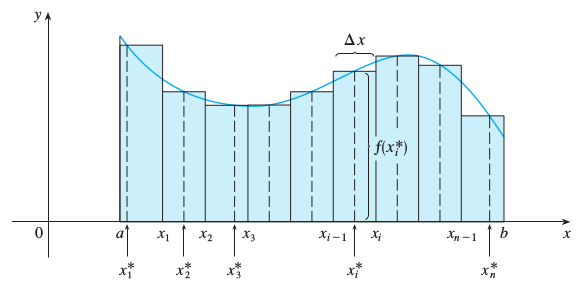
\includegraphics[scale=0.35]{imagens/int01.png}}\\
      \footnotesize{James Stewart: \emph{Cálculo} (8ª ed.,\ vol.\ 2, pg.\ 884)}
    \end{center}
  \end{figure}
  \begin{equation}
    A \approx \sum_{i=1}^n f(x_i^*) \Delta x
  \end{equation}
  \begin{equation}
    A  = \lim_{n \to \infty} \sum_{i=1}^n f(x_i^*) \Delta x = \int_a^b
    f(x) \diff x
  \end{equation}
\end{frame}

%%% Enxergando as integrais duplas
\begin{frame}
  \frametitle{Integrais duplas e volumes: visualização}
  \only<1>{
  \begin{figure}[H]
    \begin{center}
      %\caption{}
      \label{fig:int2-01}
      \fbox{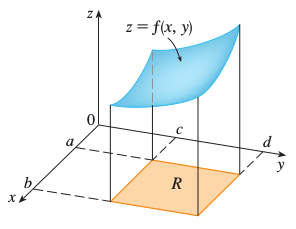
\includegraphics[scale=0.4]{imagens/int02.png}}\\
      \footnotesize{James Stewart: \emph{Cálculo} (8ª ed.,\ vol.\ 2, pg.\ 884)}
    \end{center}
  \end{figure}
  \begin{itemize}
    \item $x$ varia de $a$ até $b$
    \item $y$ varia de $c$ até $d$
    \item $x$ e $y$ formam a base, a região retangular $R$, com área $A$
    \item $z = f(x, y)$ determina uma superfície acima da região $R$
    \item $x$, $y$ e $z$ determinam um sólido $S$ com volume $V$
    \item Qual o \emph{volume} desse sólido?
  \end{itemize}
  }
  \only<2>{
    \begin{figure}[H]
      \begin{center}
        %\caption{}
        \label{fig:int2-02}
        \fbox{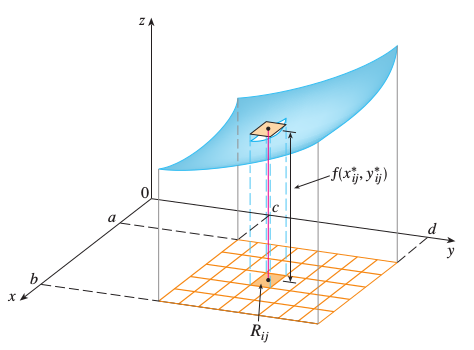
\includegraphics[scale=0.3]{imagens/int03.png}}\\
        \footnotesize{James Stewart: \emph{Cálculo} (8ª ed.,\ vol.\ 2, pg.\ 885)}
      \end{center}
    \end{figure}
    \begin{itemize}
      \item Dividimos a base retangular $R$ em vários retângulos menores: $R_{ij}$
      \item A área de cada $R_{ij}$ é: $\Delta A = \Delta x \Delta y$
      \item A altura de cada retângulo é: $f(x_{ij}^*, y_{ij}^*)$
    \end{itemize}
    \vspace{0.2cm}
    \begin{equation}
      V_{R_{ij}} \approx f(x_{ij}^*, y_{ij}^*) \Delta A
    \end{equation}
  }
  \only<3>{
    \begin{figure}[H]
      \begin{center}
        %\caption{}
        \label{fig:int2-03}
        \fbox{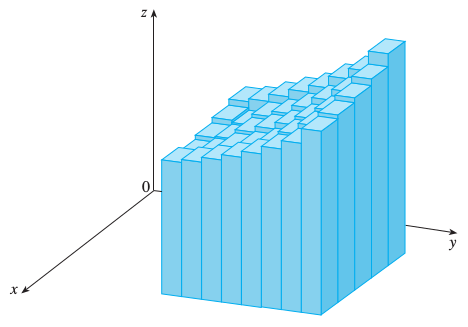
\includegraphics[scale=0.3]{imagens/int04.png}}\\
        \footnotesize{James Stewart: \emph{Cálculo} (8ª ed.,\ vol.\ 2, pg.\ 885)}
      \end{center}
    \end{figure}
    \stepcounter{equation}
    \begin{equation}
      V \approx \sum_{i=1}^m \sum_{j=1}^n f(x_{ij}^*, y_{ij}^*) \Delta A
    \end{equation}
    \begin{equation}
      V = \lim_{m, n \to \infty} \sum_{i=1}^m \sum_{j=1}^n f(x_{ij}^*,
      y_{ij}^*) \Delta A = \iint\displaylimits_R f(x, y) \diff A =
      \int_a^b \int_c^d f(x, y) \diff y \diff x
    \end{equation}
  }
  \only<4>{
    \begin{figure}[H]
      \begin{center}
        %\caption{}
        \label{fig:int2-03}
        \fbox{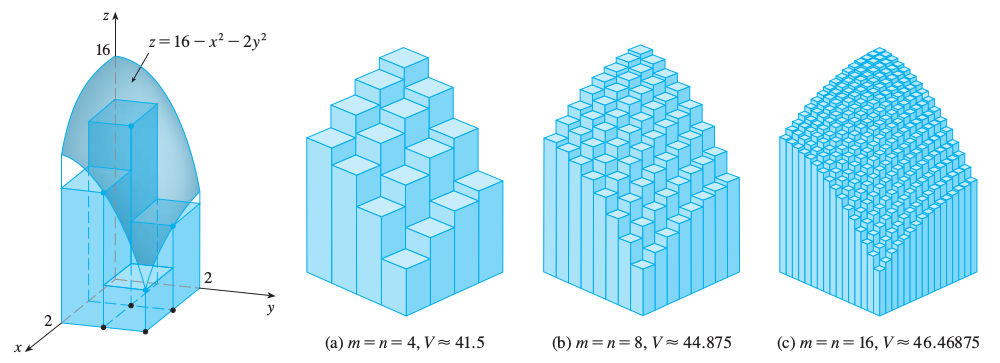
\includegraphics[scale=0.35]{imagens/int05_06.png}}\\
        \footnotesize{James Stewart: \emph{Cálculo} (8ª ed.,\ vol.\ 2, pg.\ 885)}
      \end{center}
    \end{figure}
    \begin{equation*}
      \int_{0}^{2} \int_{0}^{2} \left(16 - x^2 - 2y^2\right) \diff y \diff x = 48
    \end{equation*}
  }
\end{frame}



%%%%%%%%%%%%%%%%%%%%%%%%%%%%%%%%%%%%%%%%%%%%%%%%%%%%%%%%%%%%%%%%%%%%%%%%%%%%%%%
%%% Seção: onde a coisa complica
\section{Onde a coisa complica e qual a solução?}

\stepcounter{equation}
\stepcounter{equation}
\stepcounter{equation}

%%% Cálculo do volume sobre um disco
\begin{frame}[t]
  \frametitle{Como calcular esse volume?}
  Qual o volume do sólido limitado abaixo pelo plano $z = 0$ 
  e acima pelo parabolóide $z = 1 - x^2 - y^2$?
  \begin{columns}
    \column{0.5\textwidth}
    \centering
  \begin{figure}[H]
    \begin{center}
      %\caption{Área sob funções: integral simples}
      \label{fig:int2-04}
      \fbox{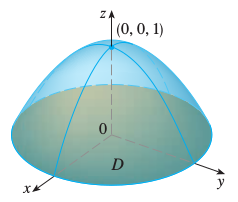
\includegraphics[scale=0.5]{imagens/int07.png}}\\
      \footnotesize{James Stewart: \emph{Cálculo} (8ª ed.,\ vol.\ 2, pg.\ 906)}
    \end{center}
  \end{figure}
    \column{0.5\textwidth}
  \begin{equation}
    \begin{split}
      V &= \iint\displaylimits_D (1-x^2-y^2) \diff A\\
        &= \int_{-1}^1 \int_{-\sqrt{1-x^2}}^{\sqrt{1-x^2}}(1-x^2-y^2)
      \diff y \diff x\\
        &=\ \text{\textbf{vixe!, complicou\ldots}}
    \end{split}
  \end{equation}
  \end{columns}
\end{frame}

%%% Por que complicou?
\begin{frame}[t]
  \frametitle{Por que complicou? Culpa de Descartes!}
  \begin{columns}
    \column{0.5\textwidth}
    \centering
    \begin{figure}[H]
      \begin{center}
        %\caption{Área sob funções: integral simples}
        \label{fig:int2-05}
        \fbox{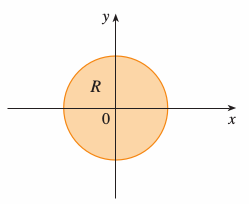
\includegraphics[scale=0.5]{imagens/int08.png}}\\
        \footnotesize{James Stewart: \emph{Cálculo} (8ª ed.,\ vol.\ 2, pg.\ 904)}
      \end{center}
    \end{figure}
    \column{0.5\textwidth}
      \begin{itemize}
        \item Nosso referencial, até agora foi o sistema de \emph{coordenadas
              retangulares} (ou cartesianas)
        \item Aqui, o disco formado por $x$ e $y$ não pode ser descrito por
              uma única função integrável: $y$ não é $f(x)$
        \item Algum corajoso aí para integrar quebrando a função em duas?
              Por simetria? E depois, como considerar o eixo $z$?
      \end{itemize}
  \end{columns}
\end{frame}

%%% Como resolver? Mudar o ponto de vista!
\begin{frame}[t]
  \frametitle{Como resolver?}
  \begin{columns}
    \column{0.5\textwidth}
    \centering
  \begin{block}{\textbf{Basta mudar o ponto de vista!}}
    \begin{figure}[H]
      \begin{center}
        %\caption{Área sob funções: integral simples}
        \label{fig:int2-06}
        \href{run:imagens/pview.mp4}{
        \fbox{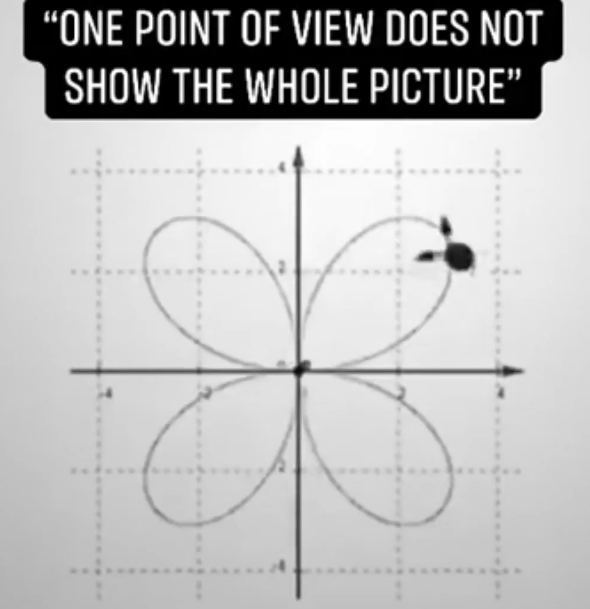
\includegraphics[scale=0.2]{imagens/int09.png}}}\\
        \footnotesize{\url{www.youtube.com/watch?v=Dmc3mQ87GiQ}}
      \end{center}
    \end{figure}
  \end{block}
    \column{0.5\textwidth}
    \centering
    \begin{itemize}
    \item Sai Descartes e o sistema de coordenadas retangulares
    \end{itemize}
    \vspace{1cm}
    \begin{itemize}
    \item Entra Newton e o sistema de \emph{coordenadas polares}
    \end{itemize}
  \end{columns}
\end{frame}


%%%%%%%%%%%%%%%%%%%%%%%%%%%%%%%%%%%%%%%%%%%%%%%%%%%%%%%%%%%%%%%%%%%%%%%%%%%%%%%
%%% Seção: Sistema de coordenadas polares
\section{Sistema de coordenadas polares}

%%% Sistema de coordenadas polares
\begin{frame}[t]
  \frametitle{Sistema de coordenadas polares}
  \begin{columns}
    \column{0.5\textwidth}
    \centering
    \begin{figure}[H]
      \begin{center}
        %\caption{}
        \label{fig:int2-07}
        \fbox{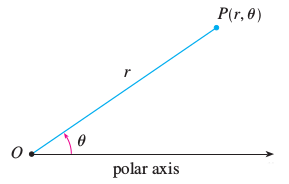
\includegraphics[scale=0.65]{imagens/int10.png}}\\
        \footnotesize{James Stewart: \emph{Cálculo} (8ª ed.,\ vol.\ 2, pg.\ 596)}
      \end{center}
    \end{figure}
    \column{0.5\textwidth}
    \begin{itemize}
      \item Especialmente útil para curvas com ``afinidade pela
            origem'', como a trajetória de um planeta
      \item Essas curvas são mais facilmente descritas como a
            trajetória de um ponto móvel cuja posição é especificada
            pela sua \emph{direção} a partir da origem e sua
            \emph{distância} da origem
      \item A direção é dada pelo ângulo $\theta$, em radianos, e a
            distância $r$ é calculada da origem até o ponto
      \item O par ordenado $P=(r,\theta)$ são as \emph{coordenadas
            polares} do ponto
    \end{itemize}
  \end{columns}
\end{frame}

%%% Características das coordenadas polares
\begin{frame}[t]
  \frametitle{Características das coordenadas polares}
  \begin{columns}
    \column{0.5\textwidth}
    \centering
    \begin{figure}[H]
      \begin{center}
        %\caption{}
        \label{fig:int2-08}
        \fbox{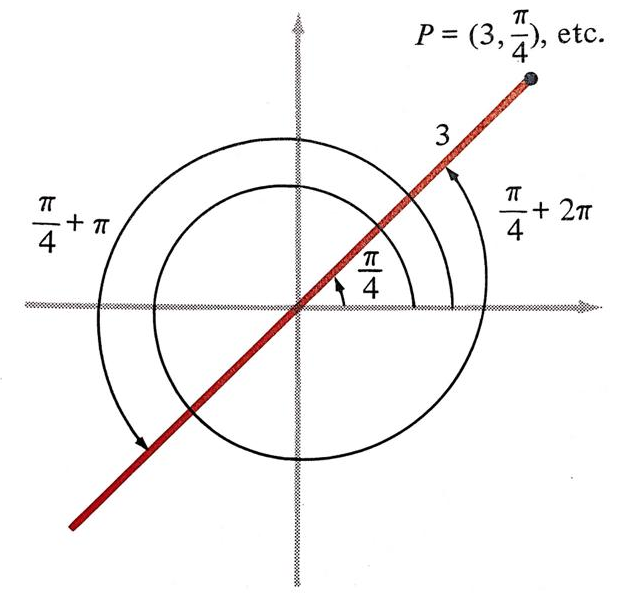
\includegraphics[scale=0.25]{imagens/int11.png}}\\
        \footnotesize{George Simmons: \emph{Calculus with Analytic
            Geometry} (2ª ed.,\ pg.\ 560)}
      \end{center}
    \end{figure}
    \column{0.5\textwidth}
    \begin{itemize}
      \item $P=(r,\theta)$ determina um ponto único, mas um ponto não
            determina uma coordenada polar única (cada ponto tem
            muitas coordenadas polares)
      \item $r=0$ especifica a origem, independente de $\theta$
      \item $(-r, \theta) = (r, \theta + \pi)$
    \end{itemize}
  \end{columns}
\end{frame}

%%% O sistema de coordenadas polares
\begin{frame}[t]
  \frametitle{O sistema de coordenadas polares}
  \begin{columns}
    \column{0.5\textwidth}
    \centering
    \begin{figure}[H]
      \begin{center}
        %\caption{}
        \label{fig:int2-16}
        \fbox{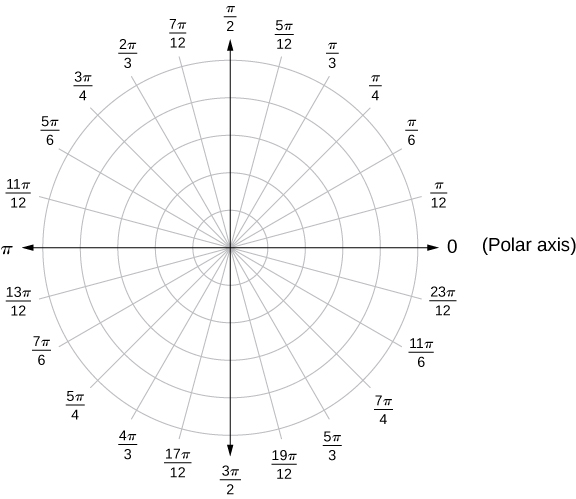
\includegraphics[scale=0.65]{imagens/int16.jpg}}\\
        \footnotesize{Gilbert Strang \& Edwin Herman: \emph{Calculus}
          (ed.\ online, 2017, vol.\ 2, pg.\ 645)}
      \end{center}
    \end{figure}
    \column{0.5\textwidth}
    \begin{itemize}
      \item Pense em termos de \emph{ao redor} e de \emph{distância}
            em relação ao centro (polo)
      \item Esqueça o pensamento cartesiano de eixo-x (esquerda e
            direita) e eixo-y (para cima e para baixo)
      \item Ao aumentarmos $\theta$ por $\pi$ ($\theta +
        \pi$) estamos na mesma ``reta'', mas na direção contrária
      \item Ao aumentarmos $\theta$ por qualquer múltiplo de
            $2\pi$ ($\theta + 2\pi$), voltamos no mesmo ponto após dar
            uma ou mais voltas
    \end{itemize}
  \end{columns}
\end{frame}

%%% Como plotar os pontos
\begin{frame}[t]
  \frametitle{Como plotar os pontos}
    \begin{figure}[H]
      \begin{center}
        %\caption{}
        \label{fig:int2-17}
        \fbox{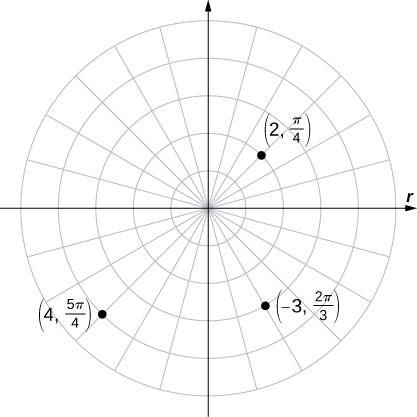
\includegraphics[scale=0.9]{imagens/int17.jpg}}\\
        \footnotesize{Gilbert Strang \& Edwin Herman: \emph{Calculus}
          (ed.\ online, 2017, vol.\ 2, pg.\ 646)}
      \end{center}
    \end{figure}
\end{frame}

%%% Equações polares
\begin{frame}[t]
  \frametitle{Curvas polares}
  \begin{block}{Gráfico de equações polares}
    O \textbf{gráfico de uma equação polar} $r = f(\theta)$ ou, mais
    genericamente, $F(r,\theta)=0$, consiste de todos os pontos $P$
    que têm \emph{pelo menos uma representação} $(r, \theta)$ cujas
    coordenadas satisfaçam a equação polar.
  \end{block}
  \begin{figure}[H]
      \begin{center}
        %\caption{}
        \label{fig:int2-11}
        \fbox{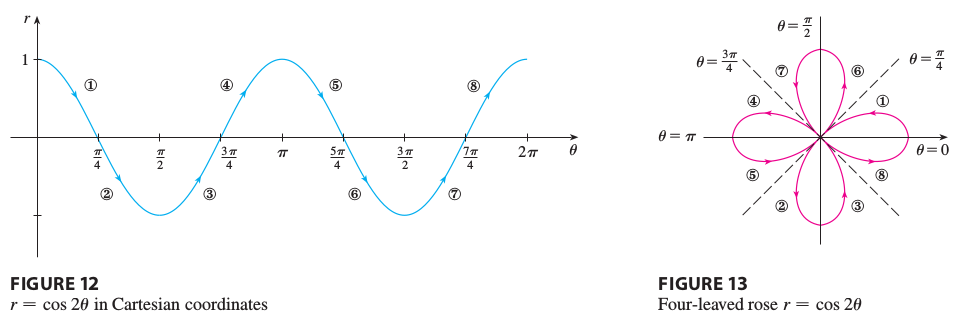
\includegraphics[scale=0.35]{imagens/int15.png}}\\
        \footnotesize{James Stewart: \emph{Cálculo} (8ª ed.,\ vol.\ 2, pg.\ 600)}
      \end{center}
    \end{figure}
\end{frame}

%%% A beleza das equações polares 1
\begin{frame}[t]
  \frametitle{A beleza polar (1): visualize, entenda e aprecie!}
  \begin{columns}
    \column{0.5\textwidth}
    \centering
    Espiral
    \begin{figure}[H]
      \begin{center}
        %\caption{}
        \label{fig:int2-18}
        \fbox{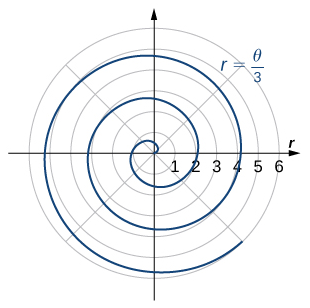
\includegraphics[scale=0.5]{imagens/int18.png}}\\
        \footnotesize{Gilbert Strang \& Edwin Herman: \emph{Calculus}
          (ed.\ online, 2017, vol.\ 2, pg.\ 651)}
      \end{center}
    \end{figure}
    \column{0.5\textwidth}
    \centering
    Cardióde
    \begin{figure}[H]
      \begin{center}
        %\caption{}
        \label{fig:int2-19}
        \fbox{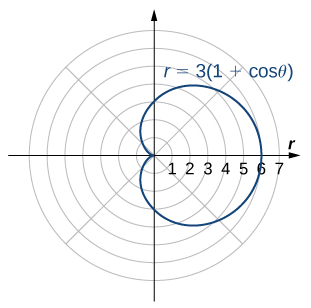
\includegraphics[scale=0.5]{imagens/int19.png}}\\
        \footnotesize{Gilbert Strang \& Edwin Herman: \emph{Calculus}
          (ed.\ online, 2017, vol.\ 2, pg.\ 652)}
      \end{center}
    \end{figure}
  \end{columns}
\end{frame}

%%% A beleza das equações polares 2
\begin{frame}[t]
  \frametitle{A beleza polar (2): visualize, entenda e aprecie!}
  \begin{columns}
    \column{0.5\textwidth}
    \centering
    Limaçon
    \begin{figure}[H]
      \begin{center}
        %\caption{}
        \label{fig:int2-20}
        \fbox{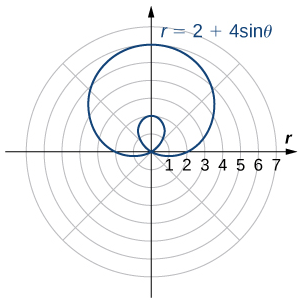
\includegraphics[scale=0.5]{imagens/int20.png}}\\
        \footnotesize{Gilbert Strang \& Edwin Herman: \emph{Calculus}
          (ed.\ online, 2017, vol.\ 2, pg.\ 652)}
      \end{center}
    \end{figure}
    \column{0.5\textwidth}
    \centering
    Rosácea
    \begin{figure}[H]
      \begin{center}
        %\caption{}
        \label{fig:int2-21}
        \fbox{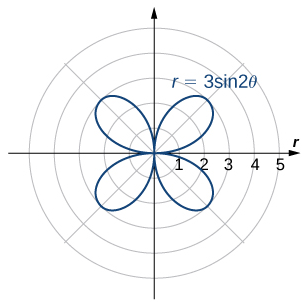
\includegraphics[scale=0.5]{imagens/int21.png}}\\
        \footnotesize{Gilbert Strang \& Edwin Herman: \emph{Calculus}
          (ed.\ online, 2017, vol.\ 2, pg.\ 652)}
      \end{center}
    \end{figure}
  \end{columns}
\end{frame}

%%% A beleza das equações polares 3
\begin{frame}[t]
  \frametitle{A beleza polar (3): visualize, entenda e aprecie!}
  \begin{columns}
    \column{0.5\textwidth}
    \centering
    \begin{figure}[H]
      \begin{center}
        %\caption{}
        \label{fig:int2-22}
        \fbox{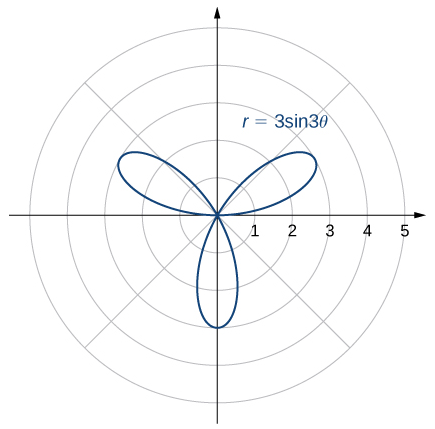
\includegraphics[scale=0.38]{imagens/int22.png}}\\
        \footnotesize{Gilbert Strang \& Edwin Herman: \emph{Calculus}
          (ed.\ online, 2017, vol.\ 2, pg.\ 652)}
      \end{center}
    \end{figure}
    \column{0.5\textwidth}
    \centering
    \begin{figure}[H]
      \begin{center}
        %\caption{}
        \label{fig:int2-23}
        \fbox{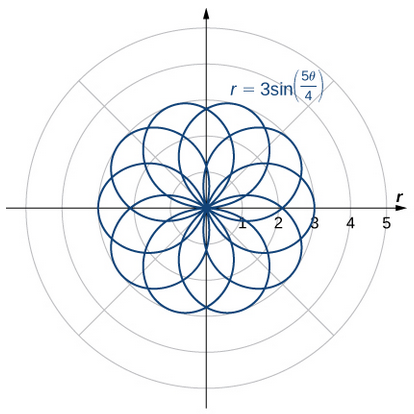
\includegraphics[scale=0.4]{imagens/int23.png}}\\
        \footnotesize{Gilbert Strang \& Edwin Herman: \emph{Calculus}
          (ed.\ online, 2017, vol.\ 2, pg.\ 652)}
      \end{center}
    \end{figure}
  \end{columns}
\end{frame}

%%% A beleza das equações polares 4
\begin{frame}[t]
  \frametitle{A beleza polar (4): visualize, entenda e aprecie!}
  \centering
  Espiral logarítmica
    \begin{figure}[H]
      \begin{center}
        %\caption{}
        \label{fig:int2-24}
        \fbox{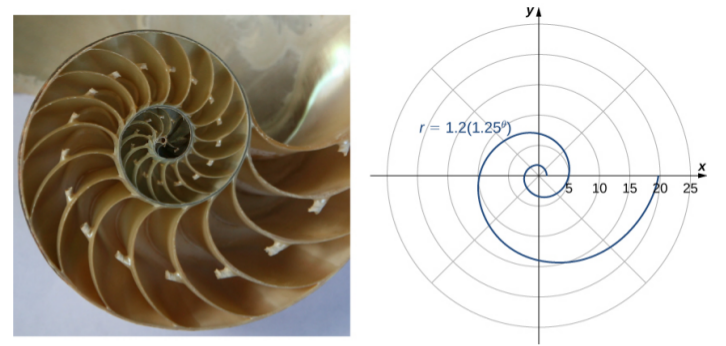
\includegraphics[scale=0.45]{imagens/int24.png}}\\
        \footnotesize{Gilbert Strang \& Edwin Herman: \emph{Calculus}
          (ed.\ online, 2017, vol.\ 2, pg.\ 655)}
      \end{center}
    \end{figure}
\end{frame}

%%% Retangular para polar e vice-versa
\begin{frame}[t]
  \frametitle{Retangular $\leftrightarrows$ Polar}
  \begin{columns}
    \column{0.5\textwidth}
    \centering
  \begin{block}{Polar para Retangular}
    \begin{equation}
      x = r \cos(\theta)
    \end{equation}
    \begin{equation}
      y = r \sin(\theta)
    \end{equation}
  \end{block}
  \begin{block}{Retangular para Polar}
    \begin{equation}
      r^2 = x^2 + y^2
    \end{equation}
    \begin{equation}
      \tan(\theta) = \frac{y}{x} \quad \therefore \quad \theta = \arctan\left(\frac{y}{x}\right)
    \end{equation}
  \end{block}
  Cuidado para que o sinal de $r$ e a escolha de $\theta$ sejam
  consistentes com o quadrante no qual o ponto $(x,y)$ está.
  \column{0.5\textwidth}
  \centering
  \begin{figure}[H]
      \begin{center}
        %\caption{}
        \label{fig:int2-25}
        \fbox{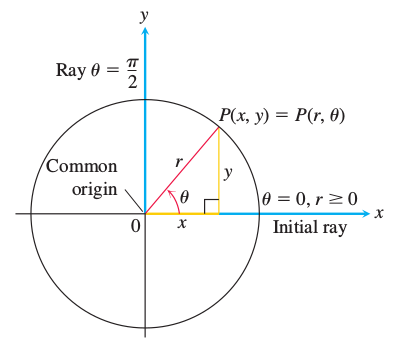
\includegraphics[scale=0.45]{imagens/int25.png}}\\
        \footnotesize{George Thomas: \emph{Thomas' Calculus: early transcedentals}
          (14ª ed., 2017, pg.\ 683)}
      \end{center}
    \end{figure}
  \end{columns}
\end{frame}

%%% Exercício: polar <--> retangular
\begin{frame}[t]
  \frametitle{Exercícios: polar para retangular e vice-versa!}
  \only<1>{
  \begin{block}{Polar para Retangular}
    \begin{figure}[H]
      \begin{center}
        %\caption{}
        \label{fig:int2-09}
        \fbox{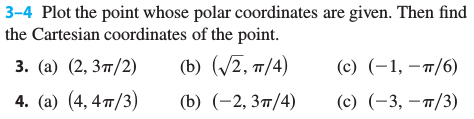
\includegraphics[scale=0.7]{imagens/int13.png}}\\
        \footnotesize{James Stewart: \emph{Cálculo} (8ª ed.,\ vol.\ 2, pg.\ 603)}
      \end{center}
    \end{figure}
  \end{block}
  }
  \only<2>{
    \begin{block}{Retangular para Polar}
    \begin{figure}[H]
      \begin{center}
        %\caption{}
        \label{fig:int2-10}
        \fbox{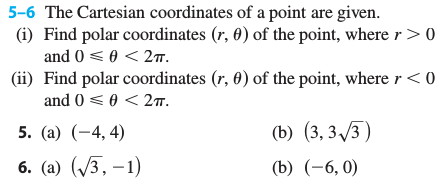
\includegraphics[scale=0.7]{imagens/int14.png}}\\
        \footnotesize{James Stewart: \emph{Cálculo} (8ª ed.,\ vol.\ 2, pg.\ 603)}
      \end{center}
    \end{figure}
  \end{block}
  }
\end{frame}


%%%%%%%%%%%%%%%%%%%%%%%%%%%%%%%%%%%%%%%%%%%%%%%%%%%%%%%%%%%%%%%%%%%%%%%%%%%%%%%
%%% Seção: Integrais simples em coordenadas polares
\section{Integrais simples em coordenadas polares}

%%% O problema da área em coordenadas polares
\begin{frame}[t]
  \frametitle{Área em coordenadas polares: como calcular?}
  Dada uma equação polar qualquer $r = f(\theta)$, como encontrar a
  área da região $R$ delimitada pelos ângulos $\theta = a$ e $\theta = b$?
  \begin{figure}[H]
    \begin{center}
      %\caption{}
      \label{fig:int1-26}
      \fbox{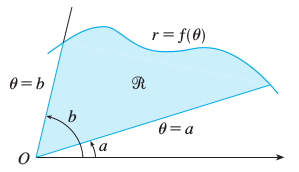
\includegraphics[scale=0.7]{imagens/int26.png}}\\
      \footnotesize{James Stewart: \emph{Cálculo} (8ª ed.,\ vol.\ 2, pg.\ 606)}
    \end{center}
  \end{figure}
\end{frame}

\setcounter{equation}{6}
%%% Dividir para conquistar
\begin{frame}[t]
  \frametitle{Mesmo raciocínio: dividir para conquistar!}
  \begin{columns}
    \column{0.5\textwidth}
    \centering
  \begin{figure}[H]
    \begin{center}
      %\caption{}
      \label{fig:int1-27}
      \fbox{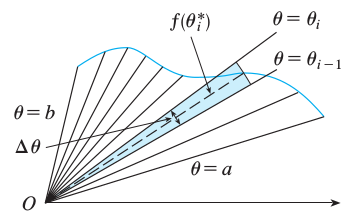
\includegraphics[scale=0.5]{imagens/int27.png}}\\
      \footnotesize{James Stewart: \emph{Cálculo} (8ª ed.,\ vol.\ 2, pg.\ 606)}
    \end{center}
  \end{figure}
  \begin{equation}
    \begin{split}
      \Delta A_i &\approx \frac{1}{2}\color{red}r\color{black}^2 \Delta \theta\\
          &\approx \frac{1}{2}\left[\color{red}f(\theta_i^*)\color{black}\right]^2 \Delta \theta
    \end{split}
  \end{equation}
  \column{0.5\textwidth}
  \centering
  \begin{figure}[H]
      \begin{center}
        %\caption{}
        \label{fig:int2-28}
        \fbox{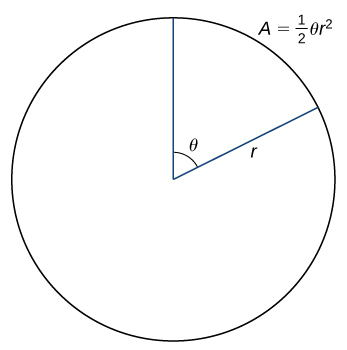
\includegraphics[scale=0.3]{imagens/int28.png}}\\
        \footnotesize{Gilbert Strang \& Edwin Herman: \emph{Calculus}
          (ed.\ online, 2017, vol.\ 2, pg.\ 663)}
      \end{center}
  \end{figure}
  Área é proporcional ao ângulo $\theta$:
  \begin{equation}
    A = \pi r^2 \times \frac{\theta}{2\pi} = \frac{1}{2}\theta r^2
  \end{equation}
  \end{columns}
\end{frame}

%%% No limite, a integral dá a área
\begin{frame}[t]
  \frametitle{No limite, a integral e a área em coordenadas polares!}
  Dada uma equação polar qualquer $r = f(\theta)$, como encontrar a
  área da região $R$ delimitada pelos ângulos $\theta = a$ e $\theta =
  b$?
  \begin{columns}
    \column{0.5\textwidth}
    \centering
  \begin{figure}[H]
    \begin{center}
      %\caption{}
      \label{fig:int1-27b}
      \fbox{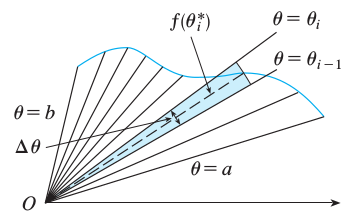
\includegraphics[scale=0.5]{imagens/int27.png}}\\
      \footnotesize{James Stewart: \emph{Cálculo} (8ª ed.,\ vol.\ 2, pg.\ 606)}
    \end{center}
  \end{figure}
  \column{0.5\textwidth}
  \centering
  \begin{equation}
    A \approx \sum_i^n \frac{1}{2}\left[f(\theta_i^*)\right]^2 \Delta \theta
  \end{equation}
  \vspace{0.5cm}
  \begin{equation}
    \begin{split}
    A &= \lim_{n \to \infty} \sum_i^n
    \frac{1}{2}\left[f(\theta_i^*)\right]^2 \Delta \theta\\
    &= \int_a^b \frac{1}{2}\left[f(\theta)\right]^2 \diff \theta\\
    &= \int_a^b \frac{1}{2}r^2 \diff \theta
    \end{split}
  \end{equation}
  \end{columns}
\end{frame}


%%%%%%%%%%%%%%%%%%%%%%%%%%%%%%%%%%%%%%%%%%%%%%%%%%%%%%%%%%%%%%%%%%%%%%%%%%%%%%%
%%% Seção: Integrais duplas em coordenadas polares
\section{Integrais duplas em coordenadas polares}

%%% Cálculo do volume sobre um disco
\begin{frame}[t]
  \frametitle{Lembra-se desta figura? Como calcular o volume agora?}
  Qual o volume do sólido limitado abaixo pelo plano $z = 0$ 
  e acima pelo parabolóide $z = 1 - x^2 - y^2$?
  \begin{columns}
    \column{0.5\textwidth}
    \centering
  \begin{figure}[H]
    \begin{center}
      %\caption{Área sob funções: integral simples}
      \label{fig:int2-04b}
      \fbox{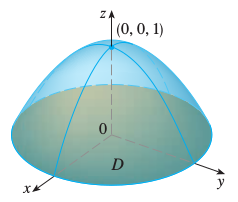
\includegraphics[scale=0.5]{imagens/int07.png}}\\
      \footnotesize{James Stewart: \emph{Cálculo} (8ª ed.,\ vol.\ 2, pg.\ 906)}
    \end{center}
  \end{figure}
    \column{0.5\textwidth}
    \centering
    \begin{itemize}
      \item Mesmo raciocínio: uma integral é a ``responsável'' pela
        área do disco, e a outra integral é a ``responsável'' pelo
        volume
        \item A diferença aqui é que 
          os cálculos da área do disco serão
          feitos com \emph{retângulos polares}!
    \end{itemize}
  \end{columns}
\end{frame}

%%% O retângulo polar
\begin{frame}
  \frametitle{Entendendo o retângulo polar}
  \centering
  $R = \{(r,\theta)\, | \, a \le r \le b, \alpha \le \theta \le \beta\}$
  \begin{figure}[H]
    \begin{center}
      %\caption{}
      \label{fig:int2-29}
      \fbox{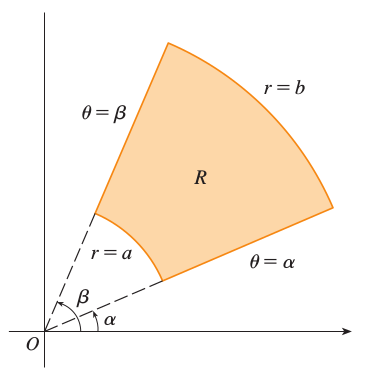
\includegraphics[scale=0.4]{imagens/int29.png}}\\
      \footnotesize{James Stewart: \emph{Cálculo} (8ª ed.,\ vol.\ 2, pg.\ 904)}
    \end{center}
  \end{figure}
\end{frame}

%%% Dividindo uma área em retângulos polares
\begin{frame}
  \frametitle{Dividindo uma área em retângulos polares}
  \begin{columns}
    \column{0.4\textwidth}
    \centering
  \begin{figure}[H]
    \begin{center}
      %\caption{}
      \label{fig:int2-30}
      \fbox{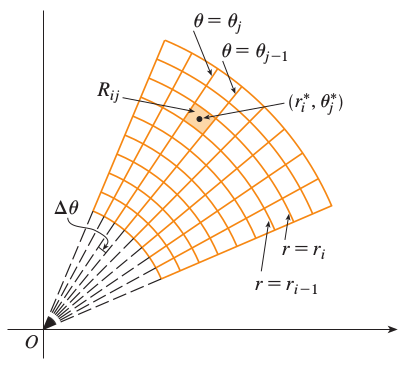
\includegraphics[scale=0.4]{imagens/int30.png}}\\
      \footnotesize{James Stewart: \emph{Cálculo}\\ (8ª ed.,\ vol.\ 2, pg.\ 904)}
    \end{center}
  \end{figure}
    \column{0.6\textwidth}
    \centering
  \begin{itemize}
    \item O intervalo $[a, b]$ é dividido em $m$ intervalos $[r_{i-1},
      r_i]$, de larguras $\displaystyle \Delta r = \frac{b-a}{m}$
    \item O intervalo $[\alpha, \beta]$ é dividido em $n$ intervalos
      $[\theta_{j-1}, \theta_j]$, de larguras $\displaystyle \Delta
      \theta = \frac{\beta - \alpha}{n}$
    \item O centro do retângulo é dado por $r_i^* = \frac{1}{2}(r_{i-1}+r_i)$ e $\theta_j^*
      = \frac{1}{2}(\theta_{j-1}+\theta_j)$
  \end{itemize}
  \vspace{0.4cm}
  \begin{equation}
    \begin{split}
      \Delta A_i &= \left(\frac{1}{2} r_i^2\Delta \theta\right) - \left(\frac{1}{2} r_{i-1}^2\Delta \theta\right)\\
                 &= \frac{1}{2}(r_i^2 - r_{i-1}^2)\Delta \theta\\
                 &= \ldots\\
                 &= \color{red}r_i^*\color{black} \Delta r \Delta \theta
    \end{split}
  \end{equation}
  \end{columns}
\end{frame}

%%% Por que retângulos e não setores?
\begin{frame}
  \frametitle{Por que retângulos e não setores?}
  \begin{columns}
    \column{0.5\textwidth}
    \centering
  \begin{figure}[H]
    \begin{center}
      %\caption{}
      \label{fig:int2-30b}
      \fbox{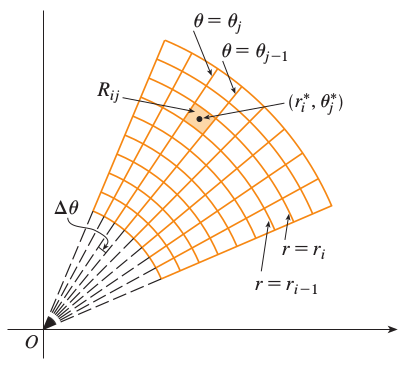
\includegraphics[scale=0.4]{imagens/int30.png}}\\
      \footnotesize{James Stewart: \emph{Cálculo}\\ (8ª ed.,\ vol.\ 2, pg.\ 904)}
    \end{center}
  \end{figure}
    \column{0.5\textwidth}
    \centering
  \begin{figure}[H]
    \begin{center}
      %\caption{}
      \label{fig:int2-27b}
      \fbox{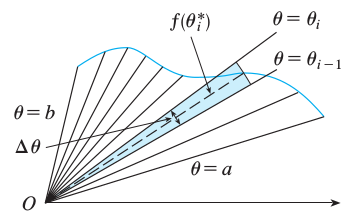
\includegraphics[scale=0.5]{imagens/int27.png}}\\
      \footnotesize{James Stewart: \emph{Cálculo}\\ (8ª ed.,\ vol.\ 2, pg.\ 606)}
    \end{center}
  \end{figure}
  \end{columns}
\end{frame}

%%% Para facilitar achar o volume!
\begin{frame}
  \frametitle{Porque queremos achar o volume!}
  \begin{columns}
    \column{0.35\textwidth}
    \centering
    \begin{equation*}
      V_{R_{ij}} \approx f[r_i^* \cos(\theta_j^*), r_i^* \sin(\theta_j^*)] \Delta A_i
    \end{equation*}
    \vspace{-1.45cm}
  \begin{figure}[H]
    \begin{center}
      %\caption{}
      \label{fig:int2-31}
      \fbox{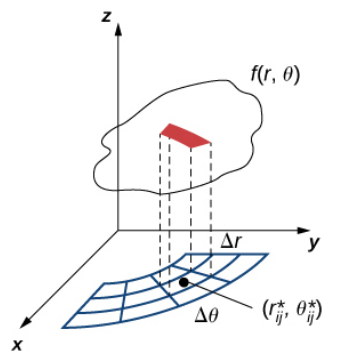
\includegraphics[scale=0.4]{imagens/int31.png}}\\
      \footnotesize{Gilbert~Strang~\&~Edwin~ Herman:\\ \emph{Calculus}
          (ed.\ online, 2017, vol.\ 3, pg.\ 527)}
    \end{center}
  \end{figure}
    \column{0.65\textwidth}
    \centering
    \begin{equation}
      \begin{split}
        V &\approx \sum_{i=1}^m \sum_{j=1}^n f[r_i^* \cos(\theta_j^*),
        r_i^* \sin(\theta_j^*)] \Delta A_i\\
          &\approx \sum_{i=1}^m \sum_{j=1}^n f[r_i^* \cos(\theta_j^*),
        r_i^* \sin(\theta_j^*)] \color{red}r_i^*\color{black}\Delta r
        \Delta \theta
      \end{split}
    \end{equation}
    \begin{equation}
      \begin{split}
        V &= \lim_{m,n \to \infty} \sum_{i=1}^m \sum_{j=1}^n f[r_i^* \cos(\theta_j^*),
          r_i^* \sin(\theta_j^*)] \Delta A_i\\
          &= \iint\displaylimits_R f[r \cos(\theta), r \sin(\theta)]
        \diff A\\
          &= \int_\alpha^\beta \int_a^b f[r \cos(\theta), r
          \sin(\theta)] \color{red}r\color{black} \diff r \diff \theta
      \end{split}
    \end{equation}
  \end{columns}
\end{frame}

%%% Exemplos de cálculos
\begin{frame}
  \frametitle{Exercícios}
  
  \begin{columns}
    \column{0.5\textwidth}
    1) Calcule $\displaystyle \iint\displaylimits_R (3x+4y^2) \diff A$, onde $R$ é a
    região no semiplano superior limitada pelos círculos $x^2 + y^2 =
    1$ e $x^2 + y^2 = 4$:
  \begin{figure}[H]
    \begin{center}
      %\caption{}
      \label{fig:int2-32}
      \fbox{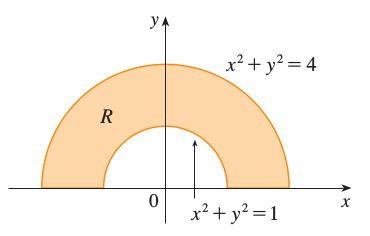
\includegraphics[scale=0.4]{imagens/int32.png}}\\
      \footnotesize{James Stewart: \emph{Cálculo}\\ (8ª ed.,\ vol.\ 2, pg.\ 904)}
    \end{center}
  \end{figure}
  
    \column{0.5\textwidth}
    2) Calcule (finalmente!) o volume do sólido limitado pelo plano $z
    = 0$ e pelo parabolóide $z = 1 - x^2 - y^2$:
  \begin{figure}[H]
    \begin{center}
      %\caption{}
      \label{fig:int2-07c}
      \fbox{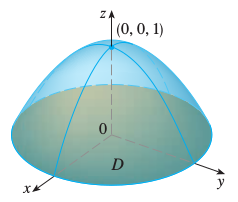
\includegraphics[scale=0.5]{imagens/int07.png}}\\
      \footnotesize{James Stewart: \emph{Cálculo}\\ (8ª ed.,\ vol.\ 2, pg.\ 906)}
    \end{center}
  \end{figure}
  
  \end{columns}
\end{frame}




%%%%%%%%%%%%%%%%%%%%%%%%%%%%%%%%%%%%%%%%%%%%%%%%%%%%%%%%%%%%%%%%%%%%%%%%%%%%%%%%
%%% Slide de encerramento com contato (descomentar se necessário)
\begin{frame}
\frametitle{Ficou com dúvida?}
\begin{center}
  \Huge Vá estudar!
  \vspace{1.6cm}
  \normalsize
  \begin{itemize}
    \item James Stewart: \emph{Cálculo}, 8ª edição, volume 2 (seções
      10.3, 10.4, 15.3)
    \item George F.\ Simmons: \emph{Calculus with Analytic Geometry},
      2ª edição (seções 16.1, 16.2, 16.3, 20.4)
    \item George B.\ Thomas, JR: \emph{Thomas' Calculus: early
      transcedentals}, 14ª (seções 11.3, 11.4, 11.5, 15.4)
    \item Gilbert Strang \& Edwin ``Jed'' Herman: \emph{Calculus},
      edição online de 2017, volume 2 (seções 7.3, 7.4)
    \item Gilbert Strang \& Edwin ``Jed'' Herman: \emph{Calculus},
      edição online de 2017, volume 3 (seções 1.3, 1.4, 5.3)
  \end{itemize}
\end{center}
\end{frame}


%%%%%%%%%%%%%%%%%%%%%%%%%%%%%%%%%%%%%%%%%%%%%%%%%%%%%%%%%%%%%%%%%%%%%%%%%%%%%%%%
%%% Encerra a apresentação!
\end{document}
